\subsection{Data Analysis Flow}

Data of DATURA has been analyzed using EUTelescope, see section before...

\label{sec:datura-nodut}
Within EUTelescope, an example set of processors and configurations were created as an introduction for new users to EUTelescope.
This example is called \texttt{datura-noDUT}, since no user DUT is included.
Two GEAR files are provided, for different telescope geometries.
No external device under test is used, only the six MIMOSA 26 telescope planes are included.
The goal of the \texttt{datura-noDUT} example is to get from raw detector data to unbiased track residuals of each telescope plane.

The \texttt{datura-noDUT} example is constructed such, that a certain sequence of steering files is called.
After all steps have been applied on a run, the unbiased residuals for this run should have been successfully calculated.

The first steering file called is the converter.
Its goal is to convert the raw MIMOSA 26 detector data into the LCIO format and remove any noisy pixels.
Following the converter, the clustering is performed.
Clusters are searched on each telescope plane and written to an LCIO collection.
A preliminary correlation is calculated and can be used for debugging purposes.
The hitmaker step transforms the clusters from two-dimensional entities on a telescope plane into hits in a global three-dimensional frame.
A rough pre-alignment is calculated and stored in a database file.

For the alignment two separate methods are available - either a simple straight line tracking or an implementation of the deterministic annealing filter (DAF) fitter~\cite{ref:daffitter}.
In both cases, the pre-alignment is loaded and applied to the hit data.
Tracks are searched and passed to \texttt{MillepedeII}~\cite{Blobel-2006} to determine the alignment constants.
These constants are then stored in another database file.

The final fitter step calculates the unbiased residual distribution for each telescope plane.
The prealignment and alignment are loaded and applied to the hit collections.
Once again, tracks are searched, but with one telescope plane considered passive, thus not contributing to the track fit.
Instead, the track is extrapolated to this plane, and the residual distance to this plane's hits is calculated.
This is repeated for each telescope plane, with histograms written to \texttt{ROOT} files.

\subsection{Geometry and multiple scattering}
\label{sec:multiplescattering}
%The telescope performance has been validated at CERN (120\,GeV pions) and DESY (1 to 6\,GeV positrons). 
%In order to get realistic data description at DESY beam energies all scattering material between sensitive planes has to be taken into account. 
%The precision of the track prediction at the DUT (plane \#3) based on five other telescope planes is shown in Figure\,\ref{fig:resolution}. 
%The combination of the thickness of the telescope planes ($\unit{50}{\upmu\meter}$) with their hit position precision ($\sim\unit{3.5}{\upmu\meter}$)
% when minimising the distances to the Detector Under Test (DUT), 
% allows to sustain track pointing precision below $\unit{3}{\upmu\meter}$ for all electron (positron) energies above 2\,GeV and distance to the DUT shorter then 20\,mm (Figure\,\ref{fig:resolution}).
%More stuff:

% (comment hjansen: actually pointing resolution! comment te: pointing only in space :) )
The figure of merit for a beam telescope is its resolution  - both in time and in space, as this defines the precision with which each track can be measured. 
The timing resolution is largely dependent on the readout speed of the used sensors, their buffer sizes and the data acquisition system. 
Spatial resolution depends on the individual intrinsic sensor resolution, the number of planes in each track and their position, as well as the multiple scattering of the beam particles. 
The expression

\begin{equation}
\label{eq:telescoperesolutionequation}
\sigma_{\textrm{meas}}^2 = \sigma_{\textrm{DUT}}^2 + \sigma_{\textrm{Tel}}^2 +
\sigma_{\textrm{MS}}^2
\end{equation}

\noindent shows the contributing terms that have to be considered~\cite{ref:eudetreport200902}. 
The measured residual width on a DUT sensor plane is expressed by $\sigma_{\textrm{meas}}$, $\sigma_{\textrm{DUT}}$ is the actual achievable resolution on the DUT plane,
 $\sigma_{\textrm{Tel}}$ is the resolution of the telescope and $\sigma_{\textrm{MS}}$ represents the contribution from multiple scattering.
In the following, all terms will be discussed.

The resolution of a telescope $\sigma_{\textrm{Tel}}$ can be expressed by

\begin{equation}
\label{eq:telescopepointing}
\sigma_{\textrm{Tel}}^2 = k \cdot \sigma_{\textrm{Intrinsic}}^2
\end{equation}

\noindent with the geometric scaling factor $k$ in turn written as

\begin{equation}
k = \frac{\sum_i^N z_i^2}{N \cdot \sum_i^N z_i^2 - \left( \sum_i^N z_i
\right)^2}
\end{equation}

\noindent assuming all $N$ telescope planes have the same intrinsic resolution $\sigma_{\textrm{Intrinsic}}$. 
$z_i$ is then the distance of the $i$-th telescope plane to the DUT positioned at $z=0$.
Multiple scattering is the term used to describe the deflection of a charged particle traversing any medium.
It depends on the particle energy and type and the radiation length of the matter traversed~\cite{ref:scatteringhighland}.
The width of the angular scattering distribution can be expressed by

\begin{equation}
\label{eq:multiplescattering}
\Theta_{0} = \frac{13.6\,\mega\electronvolt}{\beta c p} \cdot z
\sqrt{x \per X_0}
\cdot \left( 1 + 0.038 \ln{\left( x \per X_0\right) } \right)
\end{equation}

according to~\cite{ref:PDG-2014}, with the particle velocity $\beta c$, momentum $p$ and charge number $z$. 
The expression $x/X_0$ defines the thickness of the scattering medium in radiation lengths,
 with values of $X_0 = 21.82\,\allowbreak\gram\per\centi\meter^2$ for silicon and $X_0 = 36.62\,\gram\per\centi\meter^2$ for dry air, according to~\cite{ref:x0values}.

Equation~\ref{eq:multiplescattering} shows, that the angular distortion due to multiple scattering increases with the material budget and the inverse energy.
Therefore, at low-energy beams, such as the $6\,\giga\electronvolt$ DESY-II test beam, it is advantageous to have very thin telescope sensors. 
As the beam particles also interact with the atoms in the air, a contribution to the amount of multiple scattering depending on the distance between sensor planes has to be considered. 
At high-energy hadron beams ($> 100\,\giga\electronvolt$), which for example are available at the SPS facility at CERN, the contribution from multiple scattering can be neglected.

\subsection{Measurements with \Datura}

To verify the performance of the \Datura~telescope, measurements of the achievable resolution were performed in $2012$, for different settings of beam momentum,
 sensor threshold and sensor spacing~\cite{ref:thomas}.
With the \texttt{datura-noDUT} example included in the {EUTelescope} framework, which is described in detail in section~\ref{sec:datura-nodut},
 straight line tracks with hits in all six telescope planes were sought. 
From these tracks, the unbiased residual distribution of each sensor plane was calculated.
To calculate this distribution, each of the six telescope planes was iteratively considered as a DUT.
Within each iteration, tracks were calculated from the five non-DUT planes.
The unbiased residual distribution was then filled by the distance between the hit position and the track extrapolation in the DUT plane.
By using each telescope plane as a DUT, equation~\ref{eq:telescoperesolutionequation} is modified under the assumption that $\sigma_{\textrm{Intrinsic}} = \sigma_{\textrm{DUT}} = \sigma_{\textrm{M26}}$,
 leading to

\begin{equation}
\label{eq:telescoperesolutionequation_2}
\sigma_{\textrm{meas}}^2 = \sigma_{\textrm{M26}}^2 \cdot \left( 1 + k \right) +
\sigma_{\textrm{MS}}^2\,.
\end{equation}

\begin{figure}[tb]
  \centering
  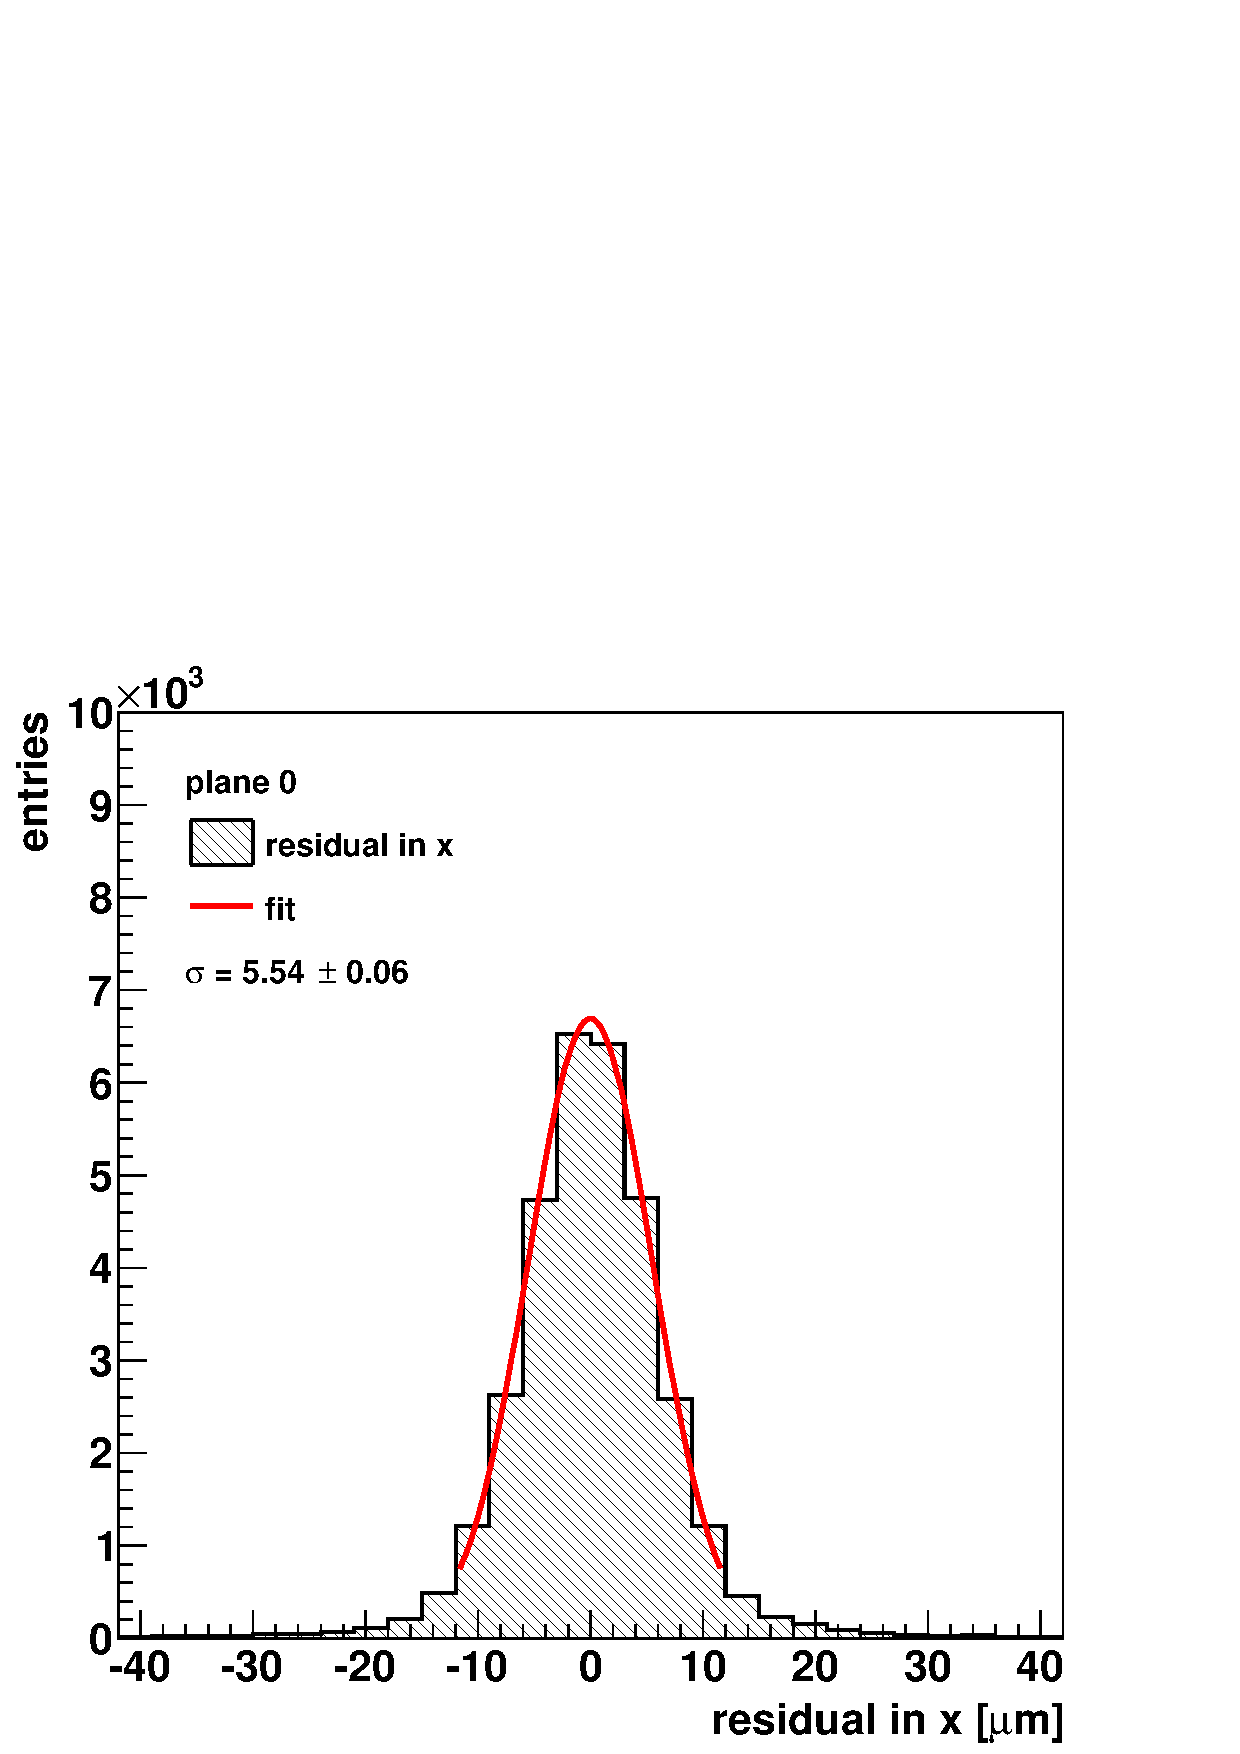
\includegraphics[width=0.45\textwidth]{figures/resis_upstream/0x.pdf}
  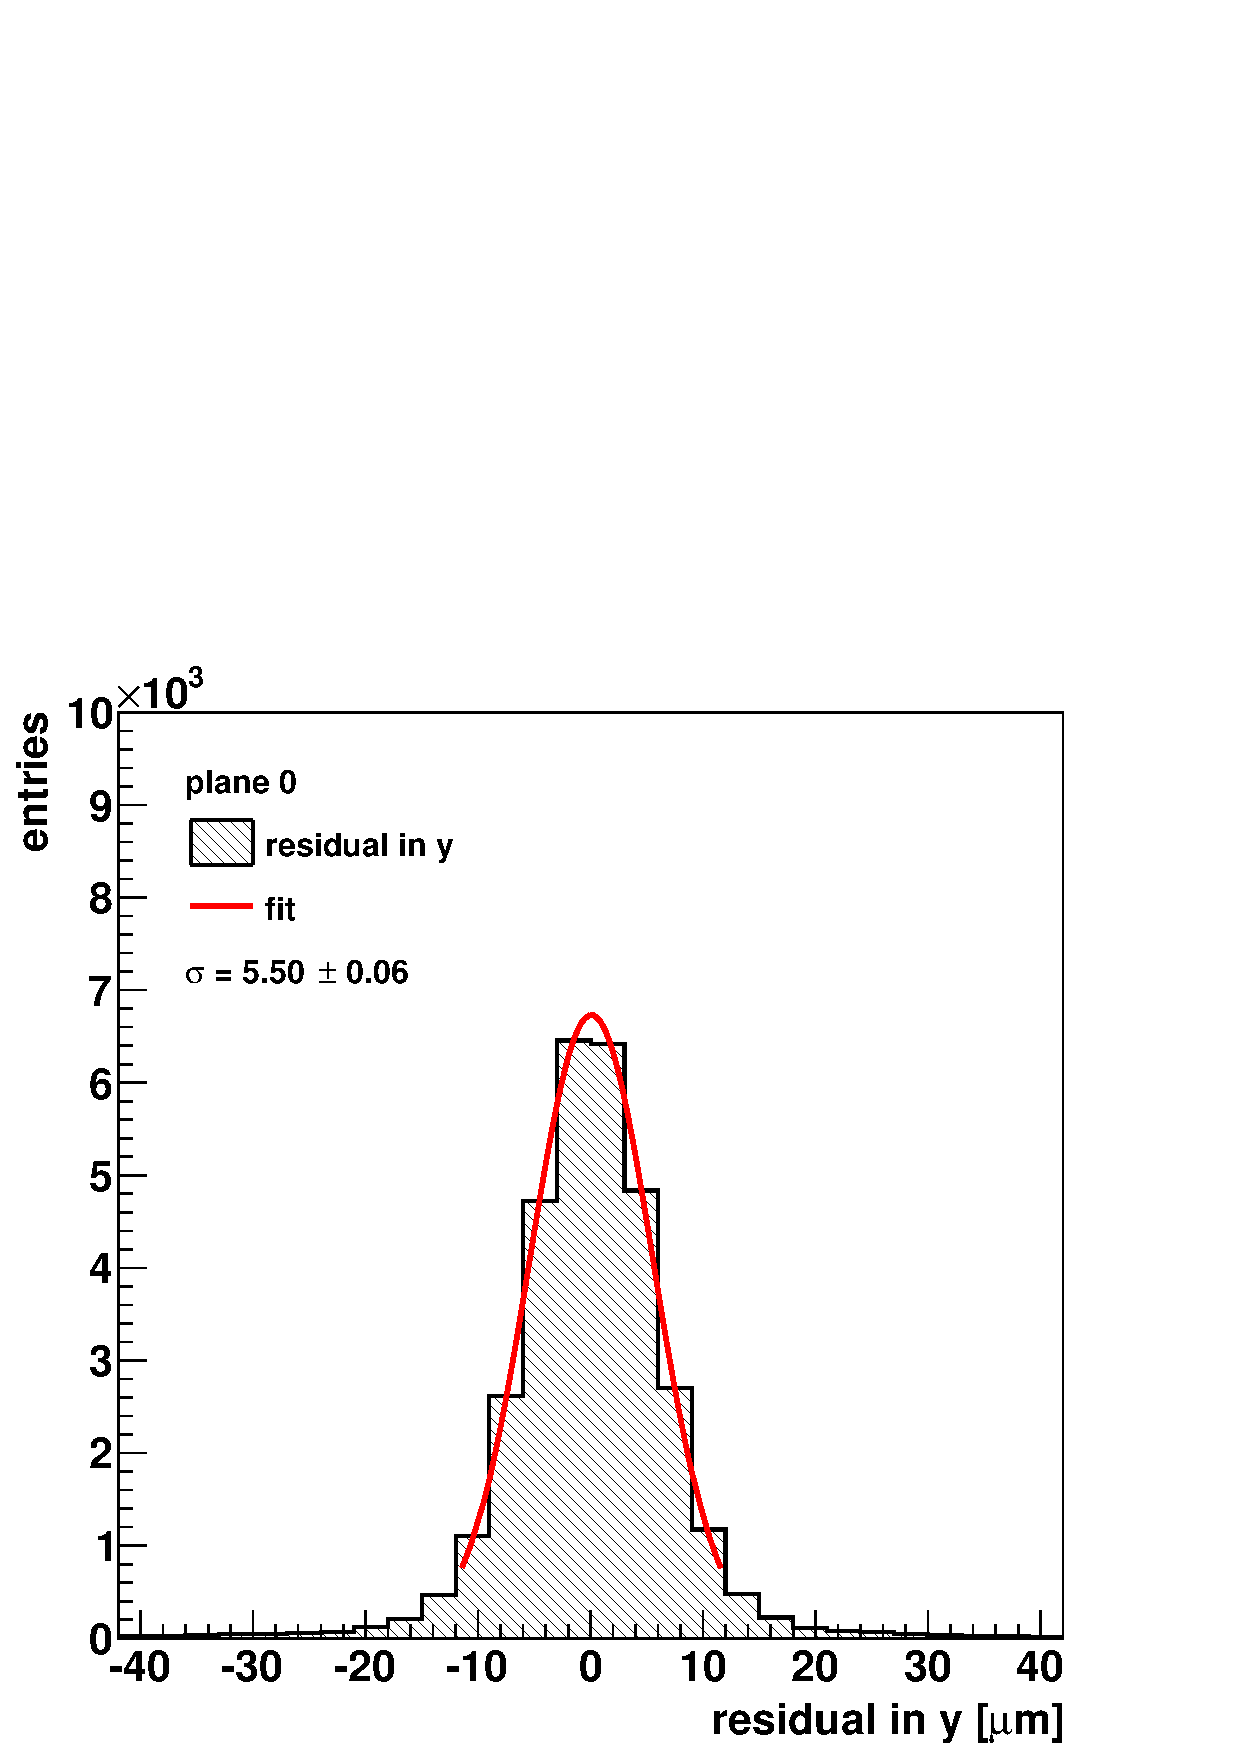
\includegraphics[width=0.45\textwidth]{figures/resis_upstream/0y.pdf}
  %\includegraphics[width=0.45\textwidth]{figures/resis_upstream/1x.pdf}
  %\includegraphics[width=0.45\textwidth]{figures/resis_upstream/1y.pdf}
  %\includegraphics[width=0.45\textwidth]{figures/resis_upstream/2x.pdf}
  %\includegraphics[width=0.45\textwidth]{figures/resis_upstream/2y.pdf}
  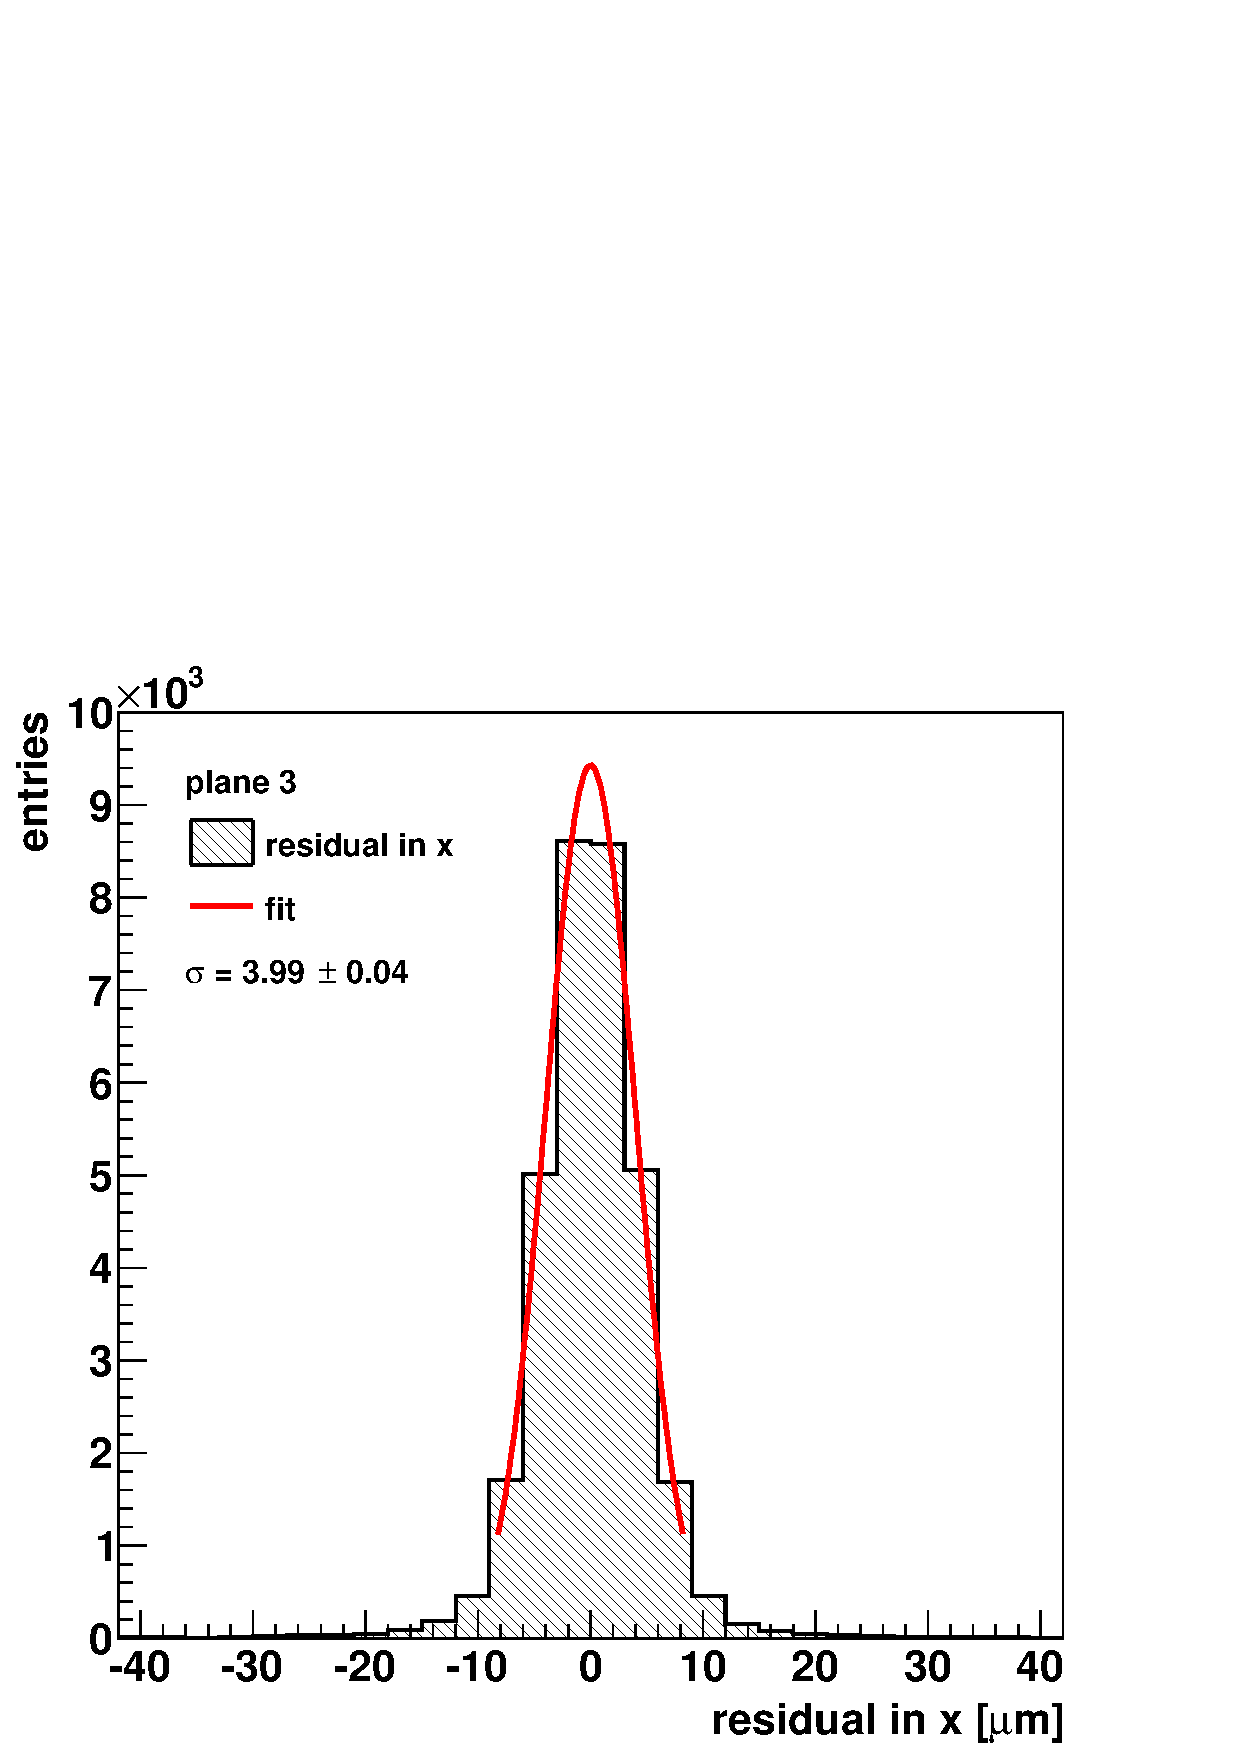
\includegraphics[width=0.45\textwidth]{figures/resis_downstream/3x.pdf}
  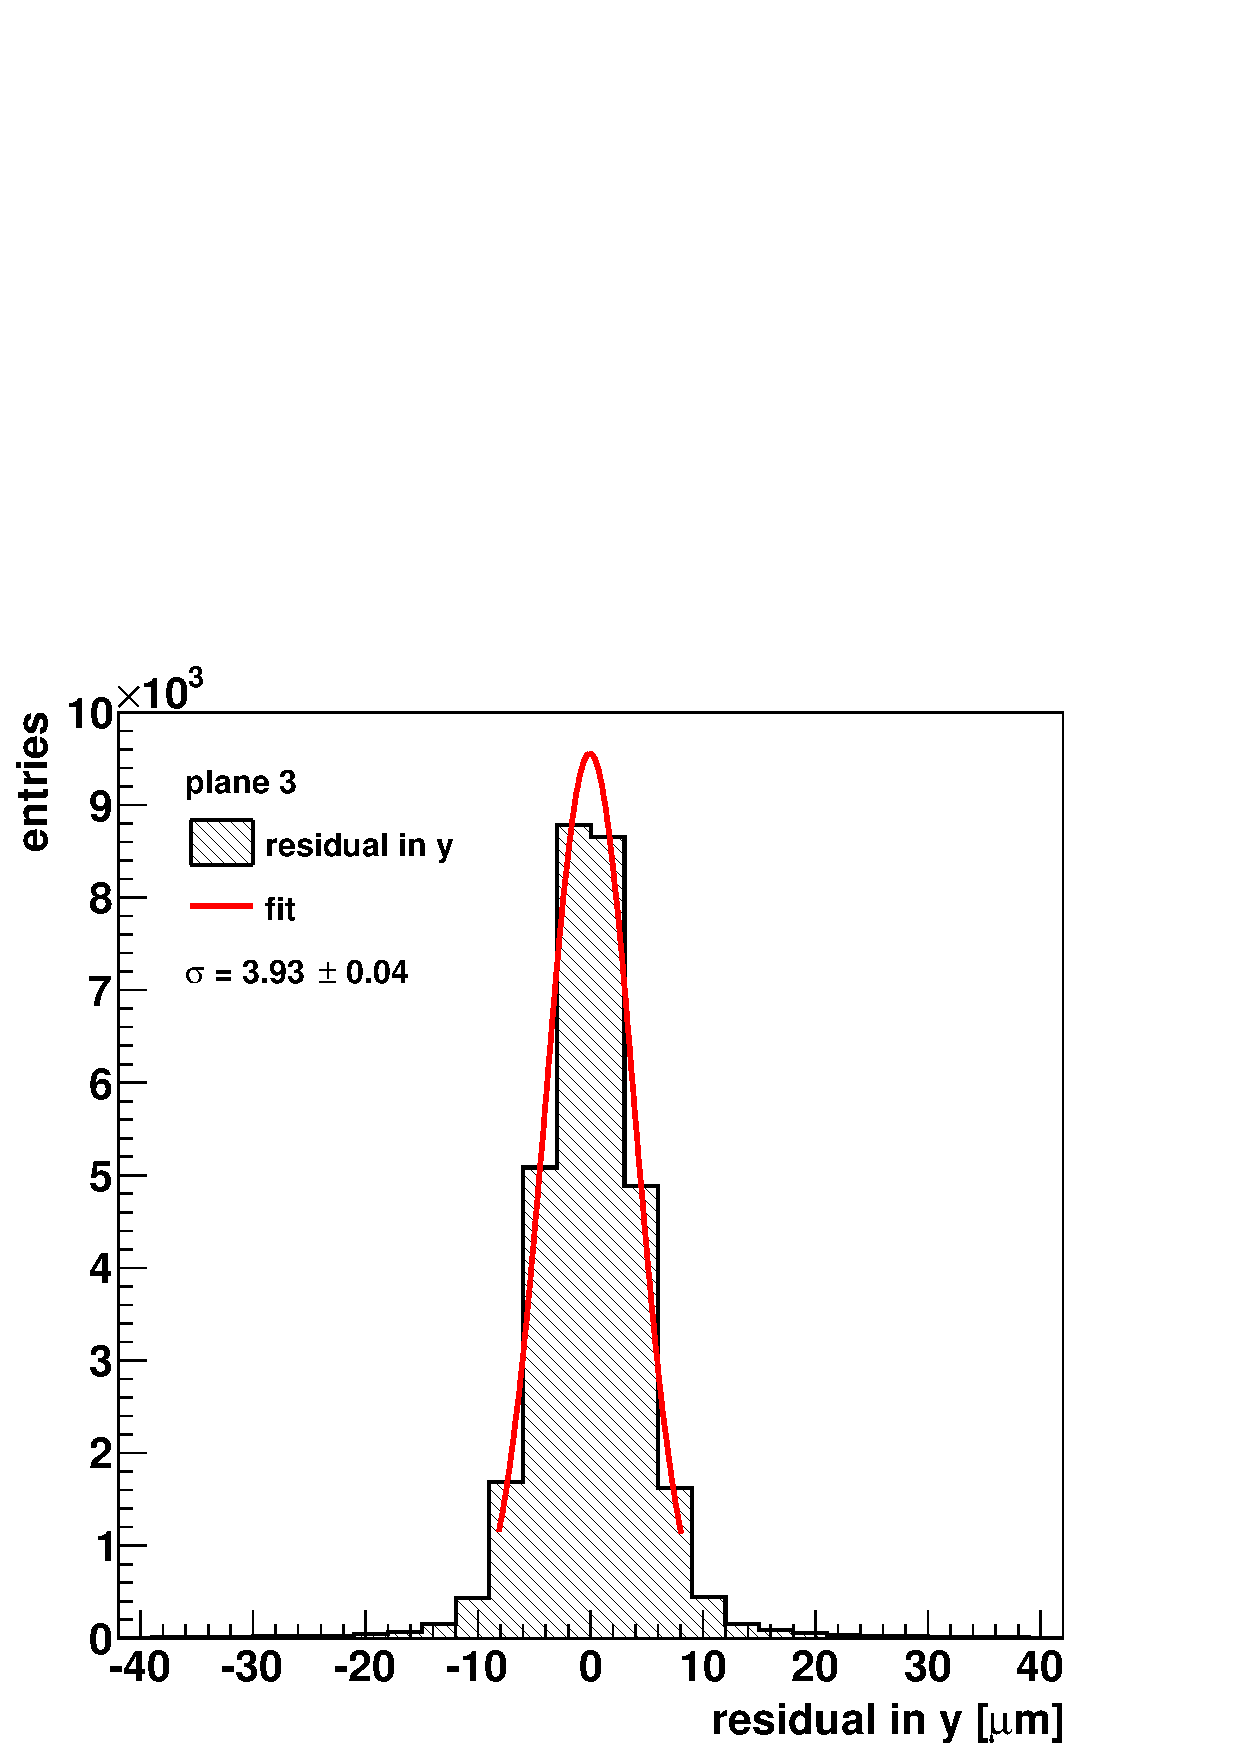
\includegraphics[width=0.45\textwidth]{figures/resis_downstream/3y.pdf}
  %\includegraphics[width=0.45\textwidth]{figures/resis_downstream/4x.pdf}
  %\includegraphics[width=0.45\textwidth]{figures/resis_downstream/4y.pdf}
  %\includegraphics[width=0.45\textwidth]{figures/resis_downstream/5x.pdf}
  %\includegraphics[width=0.45\textwidth]{figures/resis_downstream/5y.pdf}
  \caption[Residual examples to determine the \Datura telescope's resolution~\cite{ref:thomas}]{Residual examples to determine the \Datura telescope's resolution from the upstream lever arm.
From top to bottom: The measured residuals for planes $0$ and $3$, left for $x$ direction, right for $y$ direction.
Each sensor plane was considered as a passive layer during the track reconstruction. Images from~\cite{ref:thomas}.}
  \label{fig:residualexample1}
\end{figure}

Figure~\ref{fig:residualexample1} shows an example of residual distributions for a telescope sensor spacing of $20\,\milli\meter$,
 a beam momentum of $5\,\giga\electronvolt$ and a sensor threshold setting of $6$.
The residual distributions for the outer planes $0$ and $5$ are wider than the distributions obtained from the inner sensors.
This is due to the fact that the track extrapolation to the inner sensors is done from both sides, hence will be comparatively more precise than for the outer sensors,
 where the extrapolation can only be performed from one direction. 
In all cases, the distributions are fitted with a Gaussian, from which the residual width $\sigma_{\textrm{meas}}$ is determined.



% \begin{figure}[hbtp]
% \centering
% 
% \caption[Residual examples to determine the DATURA telescope's
% resolution. Downstream lever arm]{Residual examples to determine the DATURA
% telescope's resolution from the downstream lever arm. From top to bottom: The
% measured residuals for planes $3$, $4$ and $5$, left for $X$ direction, right
% for $Y$ direction. Each sensor plane was considered as a passive layer during
% the track reconstruction.}
% \label{fig:residualexample2}
% \end{figure}

By using a $\chi^{2}$ minimization method, the intrinsic resolution of the {MIMOSA 26} telescope sensors was calculated, with the contribution $\Delta \chi^2_{i,j}$ from plane $i$ in dimension $j$ defined as

\begin{equation}
\Delta \chi^2_{i,j} = \left( \frac{y_{i,j} - p_{i,j}}{\sigma_{i,j}} \right)^2 +
\left( \frac{\theta_{i,j} - \theta_{i-1,j}}{\Delta \theta_{i,j}} \right)^2 \,.
\end{equation}

\noindent The measured hit position is denoted by $y_{i,j}$, the position extrapolated from the track by $p_{i,j}$. $\theta_{i-1,j}$ and $\theta_{i,j}$ are the angles between the nominal beam direction
 and the track direction. The former is the track angle entering plane $i$, the latter the angle of the outbound track segment.
$\sigma_{i,j}$ and $\Delta \theta_{i,j}$ are the intrinsic resolution of sensor plane $i$ in dimension $j$ and the width of the multiple scattering distribution,
 according to equation~\ref{eq:multiplescattering}, respectively.
The results for both a tighter plane spacing of $20\,\milli\meter$ and a wider spacing of $150\,\milli\meter$ are shown in figure~\ref{fig:smiley}.\\

\begin{figure}[tbp]
\centering
\includegraphics[width=\textwidth]{figures/thin_smiley.pdf}
\includegraphics[width=\textwidth]{figures/wide_smiley.pdf}
\caption[Intrinsic telescope sensor resolution at $20\,\milli\meter$ and $150\,\milli\meter$ plane spacing~\cite{ref:thomas}]{Intrinsic telescope sensor resolution at $20\,\milli\meter$ (top)
 and $150\,\milli\meter$ (bottom) plane spacing.
The measured residual widths of each telescope plane are shown, for both the $x$ and $y$ axis. Dotted and dashed lines indicate the expected measurements, if a different intrinsic resolution is assumed.
The yellow band indicates the resulting intrinsic telescope sensor resolution including errors.
For both telescope geometries, data was taken at a sensor threshold setting of $6$ and with $5\,\giga\electronvolt$ electrons.
Images from~\cite{ref:thomas}.}
\label{fig:smiley}
\end{figure}

In both cases, an error of $2.5\,\milli\meter$ on the plane distance $\Delta_{\textrm{z}}$ was assumed.
The predicted intrinsic resolution $\sigma_{\textrm{M26}} = \sigma_{\textrm{Intrinsic}}$ of the MIMOSA 26 sensors is \allowbreak$\left( 3.42\,\pm\, \allowbreak 0.12 \right)\,\micro\meter$ for a plane spacing of
$20\,\milli\meter$, $\left( 3.44\,\pm\,0.10 \right)\,\micro\meter$ for a plane spacing of $150\,\milli\meter$.
For both geometries, the expected resolution of $\approx\,3.5\,\micro\meter$, according to~\cite{ref:mimosa26}, can be confirmed.
The underlying assumptions in the method presented here are:

\begin{itemize}
\item The intrinsic resolution $\sigma_{\textrm{Intrinsic}}$ of all sensor planes is assumed to be equal.
As the discriminator thresholds are set for subframes of each plane individually, however, this is not necessarily true.
Figure~\ref{fig:resivsenergy} shows the dependence of $\sigma_{\textrm{Intrinsic}}$ on the applied threshold.

\item The multiple scattering term in equation~\ref{eq:telescoperesolutionequation_2} is only calculated considering the nominal sensor thicknesses, the air between sensor planes,
 and a $25\,\micro\meter$ thick capton foil on either side of each sensor.
The particle momentum assumed is the nominal beam momentum.

\item Residuals are calculated using straight-line tracks only.
Inclined tracks, or a deflection of tracks in planes or scattering material, are not considered.
\end{itemize}

\begin{figure}[tbp]
\centering

\includegraphics[width=\textwidth]{figures/resi_thresh_errors.pdf}
\caption[Telescope intrinsic sensor resolution for different threshold settings, beam momenta and geometries~\cite{ref:thomas}]{
 The measured intrinsic resolution of the \Datura telescope's MIMOSA 26 sensors $\sigma_{\textrm{M26}}$ for different beam momenta $p$, sensor spacing $\Delta_{\textrm{z}}$ and applied sensor threshold.
Some values are shifted on the x-axis for improved legibility.
Image from~\cite{ref:thomas}.}
\label{fig:resivsenergy}
\end{figure}

Figure~\ref{fig:resivsenergy} shows the calculated intrinsic telescope sensor resolution for different beam energies, plane distances and applied sensor thresholds.
The minimum of the MIMOSA 26 sensors' intrinsic resolution is reached for a threshold setting of $6$.
While the measured residual width for wider sensor spacings or lower beam momenta is higher, as can be seen in figure~\ref{fig:smiley},
 these effects are accounted for in equation~\ref{eq:telescoperesolutionequation} by the terms $\sigma_{\textrm{Tel}}^2$ and $\sigma_{\textrm{MS}}^2$.
Because of this, the difference in intrinsic sensor resolution between configurations at any given threshold is only approximately $\pm\,0.15\,\micro\meter$, which is well within the errors.
From equation~\ref{eq:telescopepointing} the optimal track pointing resolution $\sigma_{\textrm{Tel}}$ of the \Datura telescope without multiple scattering
 can therefore be given as $\left( 1.40 \pm 0.05 \right)\,\micro\meter$.\\
Measurements by Behr~\cite{ref:j.behrmeasurements}, taken at high thresholds $>\,10$ show comparable results of $\sigma_{\textrm{M26}} = (4.35\,\pm\,0.10)\,\micro\meter$.

The signal-to-noise threshold applied to each telescope sensor is a critical parameter for a telescope's performance.
A higher threshold will cut into the signal, thus reducing the amount of clusters found on each plane and therefore reducing the amount of reconstructable tracks.
This reduces a sensor's efficiency.
A lower threshold will allow an increasing amount of noise hits to be wrongly identified as clusters.
This again will also lead to a broadening of the residual distributions.
Figure~\ref{fig:effi} shows the efficiency distribution over a sensor plane.
The efficiency is defined as the ratio of hits being measured in the vicinity of a traversing track to the overall number of tracks.
$100\,\micro\meter$ was considered as maximum distance.
A noisy pixel column at $\approx Y = -8\,\milli\meter$ can be observed.
This column was masked during the converter step in the \texttt{datura-noDUT} example and subsequently is not used during the analysis.
Disregarding this area, an overall average efficiency over $98\,\%$ is observed.

\begin{figure}[tbp]
  \centering
  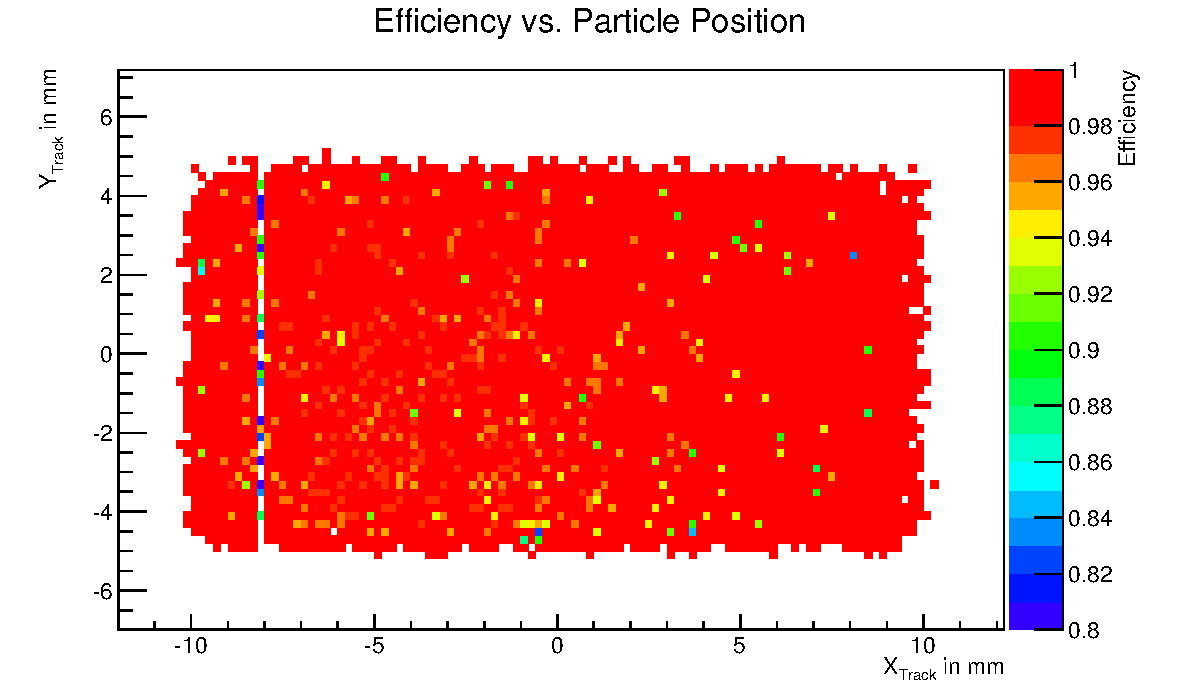
\includegraphics[width=\textwidth]{figures/plane3_effi_run37.pdf}
  \caption[Telescope sensor efficiency~\cite{ref:thomas}]{Efficiency of telescope sensor plane $3$ at a threshold of $7$ and $5\,\giga\electronvolt$ beam momentum.
Image from~\cite{ref:thomas}.}
\label{fig:effi}
\end{figure}

In figure~\ref{fig:effi_thresh}, the efficiency dependence on the sensor threshold is shown, for various beam momenta and sensor spacings.
Efficiencies are averaged for all six sensor planes and both spatial coordinates.
In all cases, the efficiency is $\ge\,98\,\%$ up to a threshold setting of 7.
With increasing threshold, the efficiency declines, until an efficiency of $86\,\%$ for threshold $12$ is reached.
The difference between momenta and plane spacings is due to multiple scattering and increased telescope resolution.

\begin{figure}[tbp]
  \centering
  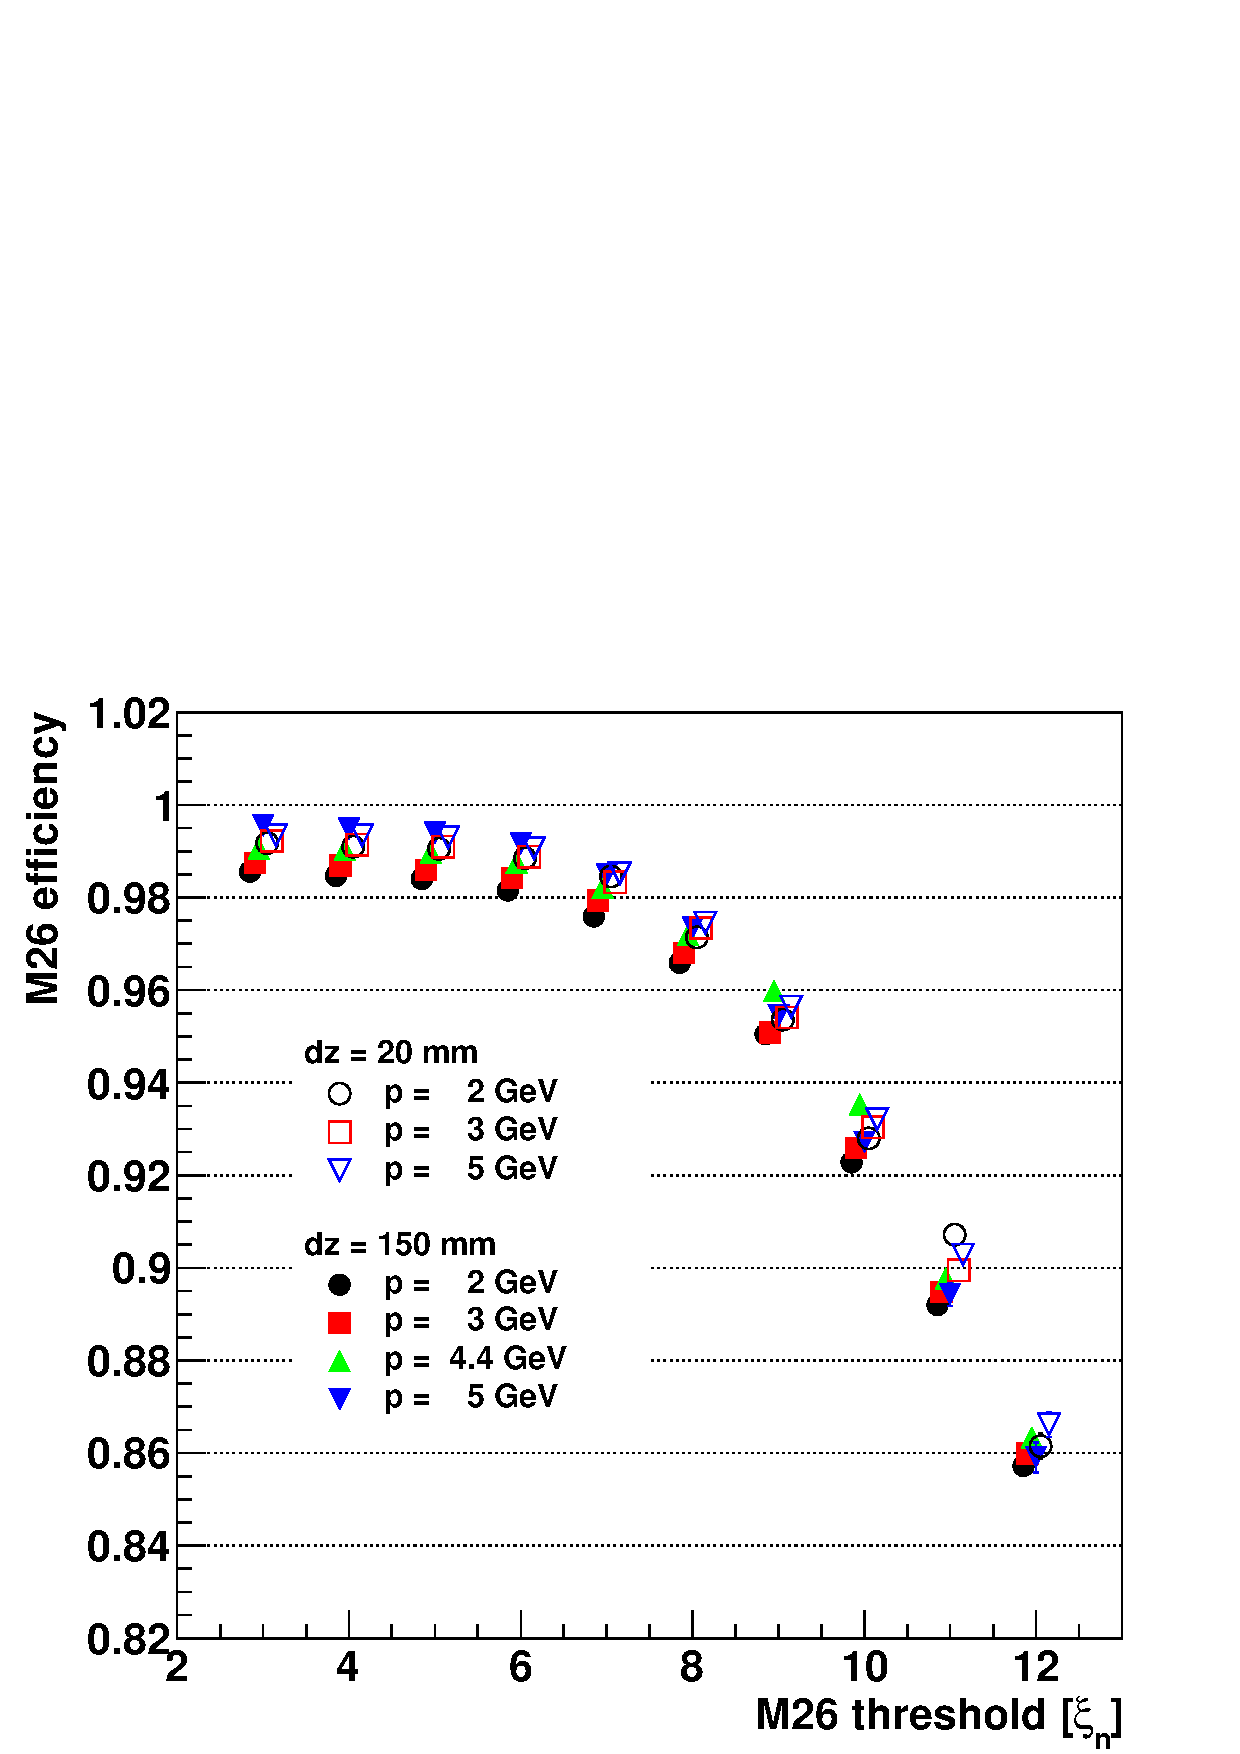
\includegraphics[width=\textwidth]{figures/effi_thresh.pdf}
  \caption[Overall telescope sensor efficiency vs. threshold for different beam momenta and sensor spacings~\cite{ref:thomas}]{
 Average efficiency of all telescope sensors in both dimensions for different beam momenta and sensor spacing vs. applied threshold.
An efficiency decline with increasing threshold can be observed.
Some values are shifted on the $x$ axis for improved legibility.
Image from~\cite{ref:thomas}.}
\label{fig:effi_thresh}
\end{figure}



\subsection{Resolution predictions using General Broken Lines}

With the measured intrinsic resolution at hand, and the knowledge about the amount of material of the sensor planes, predictions of the expected pointing resolution at the actual DUT position can be made. 
Therefore, it is possible to calculate a priori the optimal telescope geometry for a certain measurement. 
Using the GBL formalism \cite{Kleinwort-2012,Blobel-2006}, the resolution is analytically calculated at desired points of interest along the particle trajectory. 
Assuming the parameter summarised in Table~\ref{tab:parameters}, the pointing resolution at the DUT for three different DUT material budgets is plotted as a function of the spacing $dz_2$ between
 the closest planes up- and downstream of the DUT.
 
Some considerations:\\
7 dimensions: dz, dz2, dz3, $\sigma_{reso}$, $\epsilon_{\textrm{M26}} = \frac{X_{\textrm{M26}}}{X_0}$, $\epsilon_{\textrm{DUT}} = \frac{X_{\textrm{DUT}}}{X_0}$,  p in GeV\\
assume symmetric set-up: dz2 = dz3, $\sigma_{reso}$ and $\epsilon_{\textrm{M26}}$ are fixed, p is 5\,GeV and 120\,GeV, so only 3 dimensions left.



\begin{figure}[tbp]
  \centering
  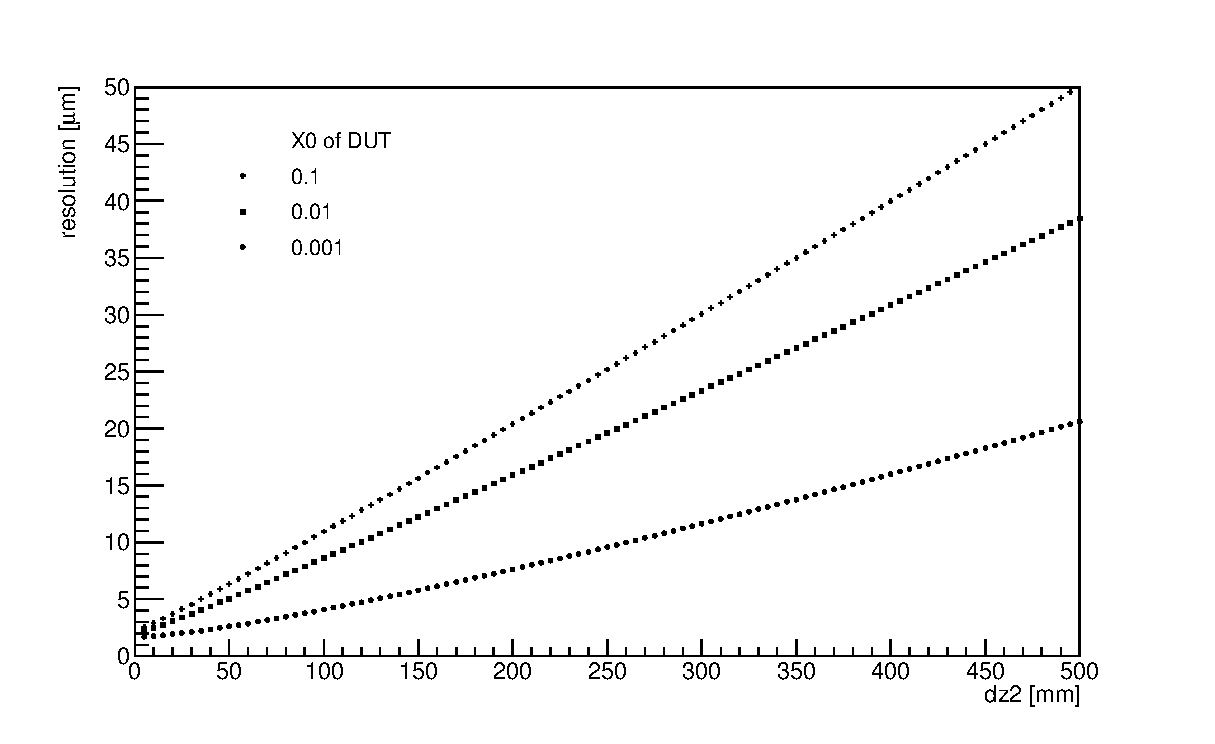
\includegraphics[width=0.49\textwidth]{figures/CalcResoAtDesy}
  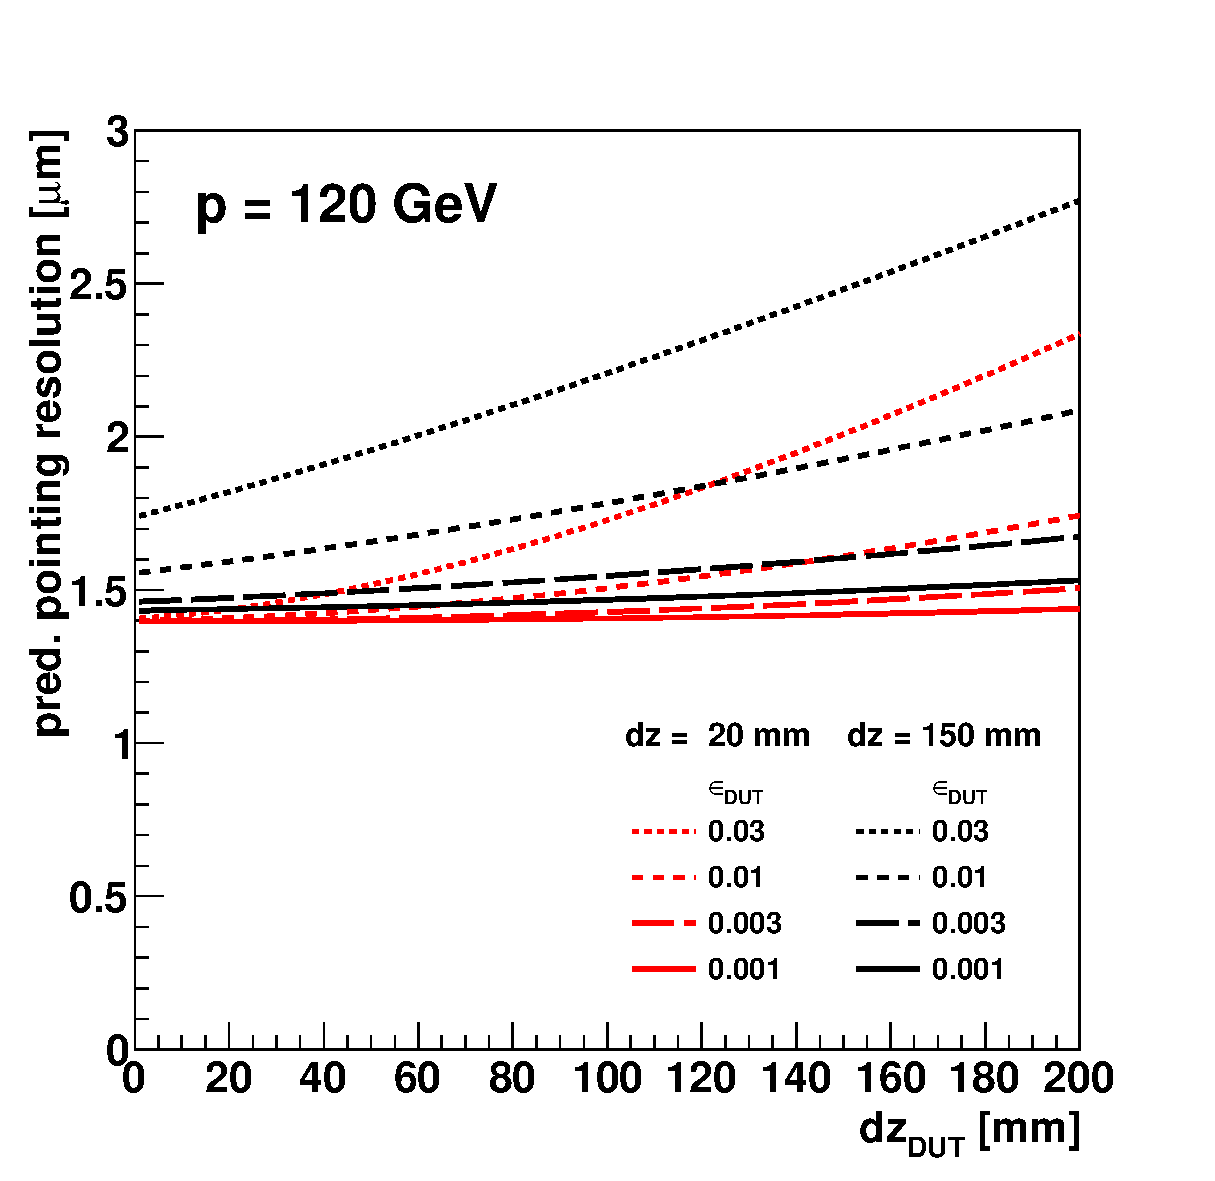
\includegraphics[width=0.49\textwidth]{figures/CalcResoAtSPS}\\
  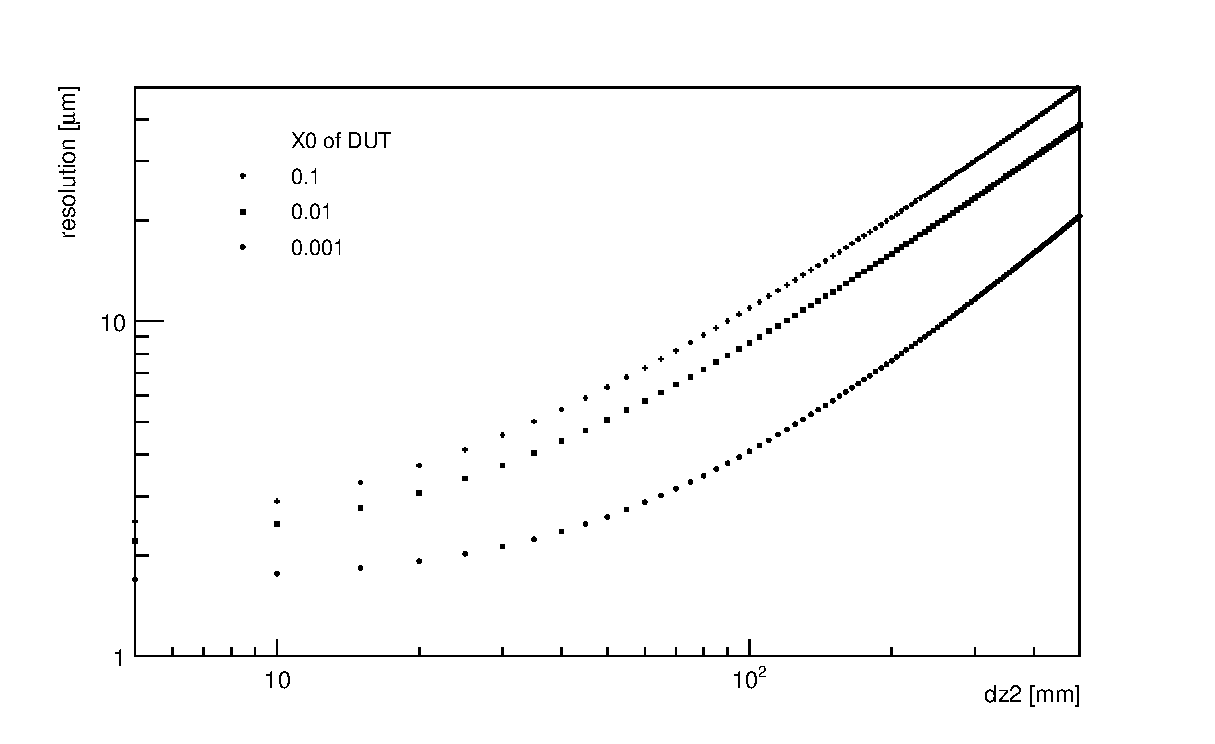
\includegraphics[width=0.49\textwidth]{figures/CalcResoAtDesy_loglog}
  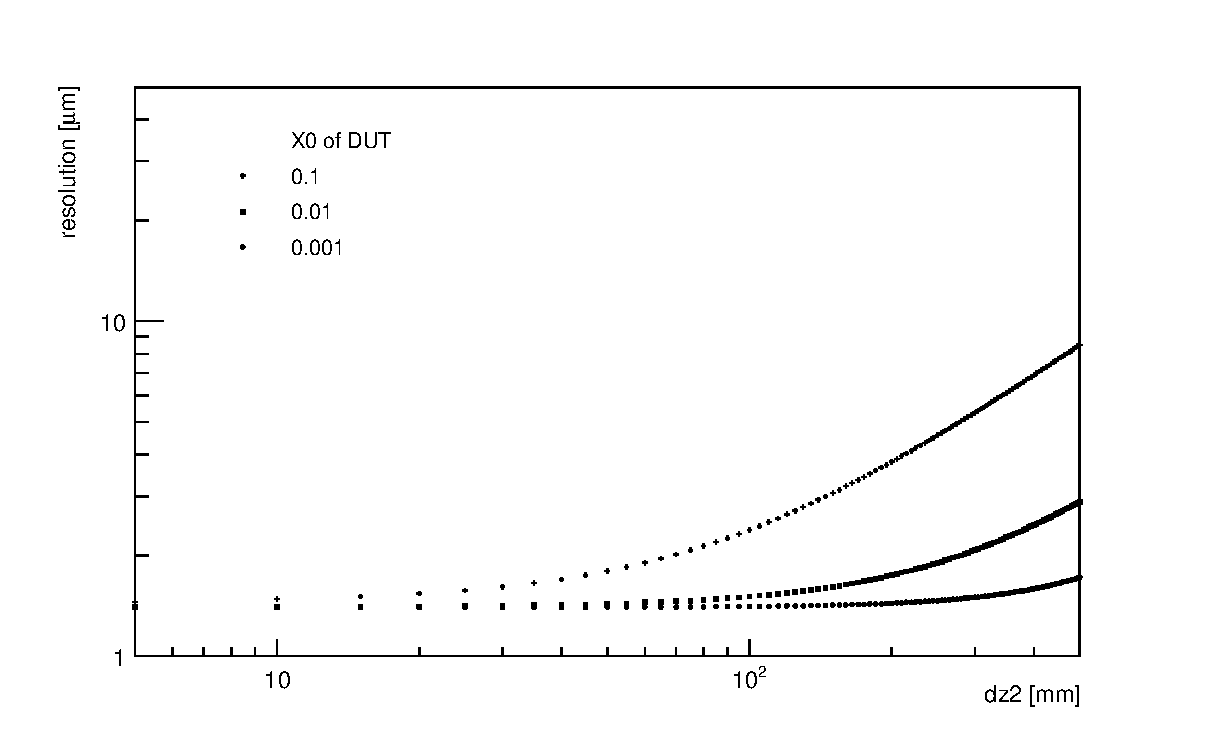
\includegraphics[width=0.49\textwidth]{figures/CalcResoAtSPS_loglog}
  \caption[Pointing resolution for various DUTs as a function of the distance between DUT and neighbouring planes]{
  The pointing resolution for various DUTs is shown as a function of the equidistant distance between DUT and neighbouring planes.
  Left: at 5\,GeV, Right: at 120\,GeV. }
\label{fig:CalcResos}
\end{figure}
